
\section{Features}
\label{sec:features}

The UCVM platform offers an API and a set of programs, many of which can be used either in a single processor context or in parallel. This section details the most relevant of these programs, categorized by the broad feature they are intended to support. The discussion will focus largely on how the single processor programs operate. Those features that have additional support for parallel computing will be noted, and any operational differences between the single core and parallel implementations shall be described.

The single-core commands can be run in any system where the platform has been successfully installed. The parallel commands, however, require a system where the standard Message Passing Interface (MPI) library and compilers are available. Single-core commands are useful to most users interested in exploring the properties of the regions covered by the models supported by the platform. On the other hand, advanced users needing to build large-scale (regional) materialized velocity models for earthquake modeling and simulation are the more likely to use the MPI commands. 

%\textcolor{green}{For each utility, we should implicitly answer four questions as a narrative. 1) What problem is this utility trying to solve? 2) How does this utility solve the problem? 3) What information does the user need to provide? 4) What does the utility output? For the input description, rather than providing a configuration file, I would use a table with the relevant parameters to the problem and a description of each (ignoring simple things like output file paths, number of processors, etc).}


% ---------------------------------------------------------------------------------------------
% TEMP FIGURE: Needs to be completed and improved in Illustrator and moved to final PDF dir.
\begin{figure*}[ht!]
	\centering
%	\includegraphics
%		[width=0.75\textwidth]
%		{figures/raw-pdf/covered-areas}
	\fbox{\begin{minipage}{\textwidth}\textcolor{red}{PENDING}\vspace{2in}\end{minipage}}
	\caption{Querying a geographic point for material properties.}
	\label{fig:tiling}
\end{figure*}
% ---------------------------------------------------------------------------------------------


\subsection{Querying Material Properties}

UCVM provides two methods for querying models. The first method is programmatically, directly through the provided C language API. The second is via the command-line program \texttt{ucvm\_query}. Both methods query the underying models in the same manner; the \texttt{ucvm\_query} program is merely a simplified front-end layered upon the API.

The query process begins with the identification of one or more CVMs as the source of material properties. In this respect, the framework distinguishes between geo-technical layers and standard crustal models, allowing the user to make selections for both. As illustrated in Figure \ref{fig:tiling}, the set of standard crustal models is tiled in three dimensions to form a meta-model. The same operation is performed on the GTLs to define a meta-GTL. The interface between the meta-GTL and meta-model is then smoothed using an interpolation function (linear interpolation in the simplest case) along a user-defined interpolation zone parallel to the z-axis. Note that when two or more models overlap in three dimensional space, the model listed first within the tiling order will satisfy requests within that overlapping zone.

Once the models have been tiled in this manner, the API or program accepts one or more input query points from the user. For every point, the framework queries each component model of the two meta models, until either a valid set of velocities and density are returned, or all component models have been queried and the request was unsatisfied. Thus, for points that fall within the interpolation zone, two sets of material properties may be generated - one each for each meta model. These two sets of material properties are then combined using the interpolation function. As the native query interfaces of available CVMs accept query points in a wide array of formats (geographic coordinates versus UTM-11 map coordinates, or depth versus elevation for the vertical component, for example), UCVM may perform a coordinate transformation to convert its input format of decimal (latitude, longitude, depth/elevation) tuples to the local coordinate system of the component model being queried. This is accomplished transparently by utilizing the standard projection library Proj.4 (NOTE: cite Proj.4).

In the case of the API, the result of a successful query is a data-structure containing the velocities $V_{p}$ and $V{s}$, and the density $\rho$ at the point of interest, along with the elevation in meters and $V_{S30}$ of the corresponding point on the free-surface, and an indication of which velocity model within the meta-model ultimately satisfied the request. For those points which fall within the interpolation zone between the meta-GTL and meta-model, the framework additionally identifies the material properties reported by the meta-GTL and meta-model, as well as the component models from which they were extracted. For the \texttt{ucvm\_query} program, this same information is formulated in tabular format and printed to the screen.

This tiling mechanism can be a powerful feature for combining multiple regional velocity models, but a problem arises when velocity models overlap in three-dimensional space. Simply tiling two overlapping models will create a three-dimensional interface that may contain sharp contrasts in either velocities or density. This artifact is undesirable for earthquake simulation applications as it can cause reflections in wavefronts. There are two approaches to remedy this problem. The simplest approach is to define a UCVM patch model to trilinearly interpolate the material properties within arbitrary cuboid geographic region. This patch model may be tiled along with the overlapping traditional velocity models to produce a smoothed meta-model. However, this numerical smoothing approach does not reflect the physical structures of the Earth's surface. The second approach is to utilize UCVM to query all models within the overlap zone individually, and then manually combine the results with a user-defined interpolation function. 


\begin{figure*}[ht!]
	\centering
	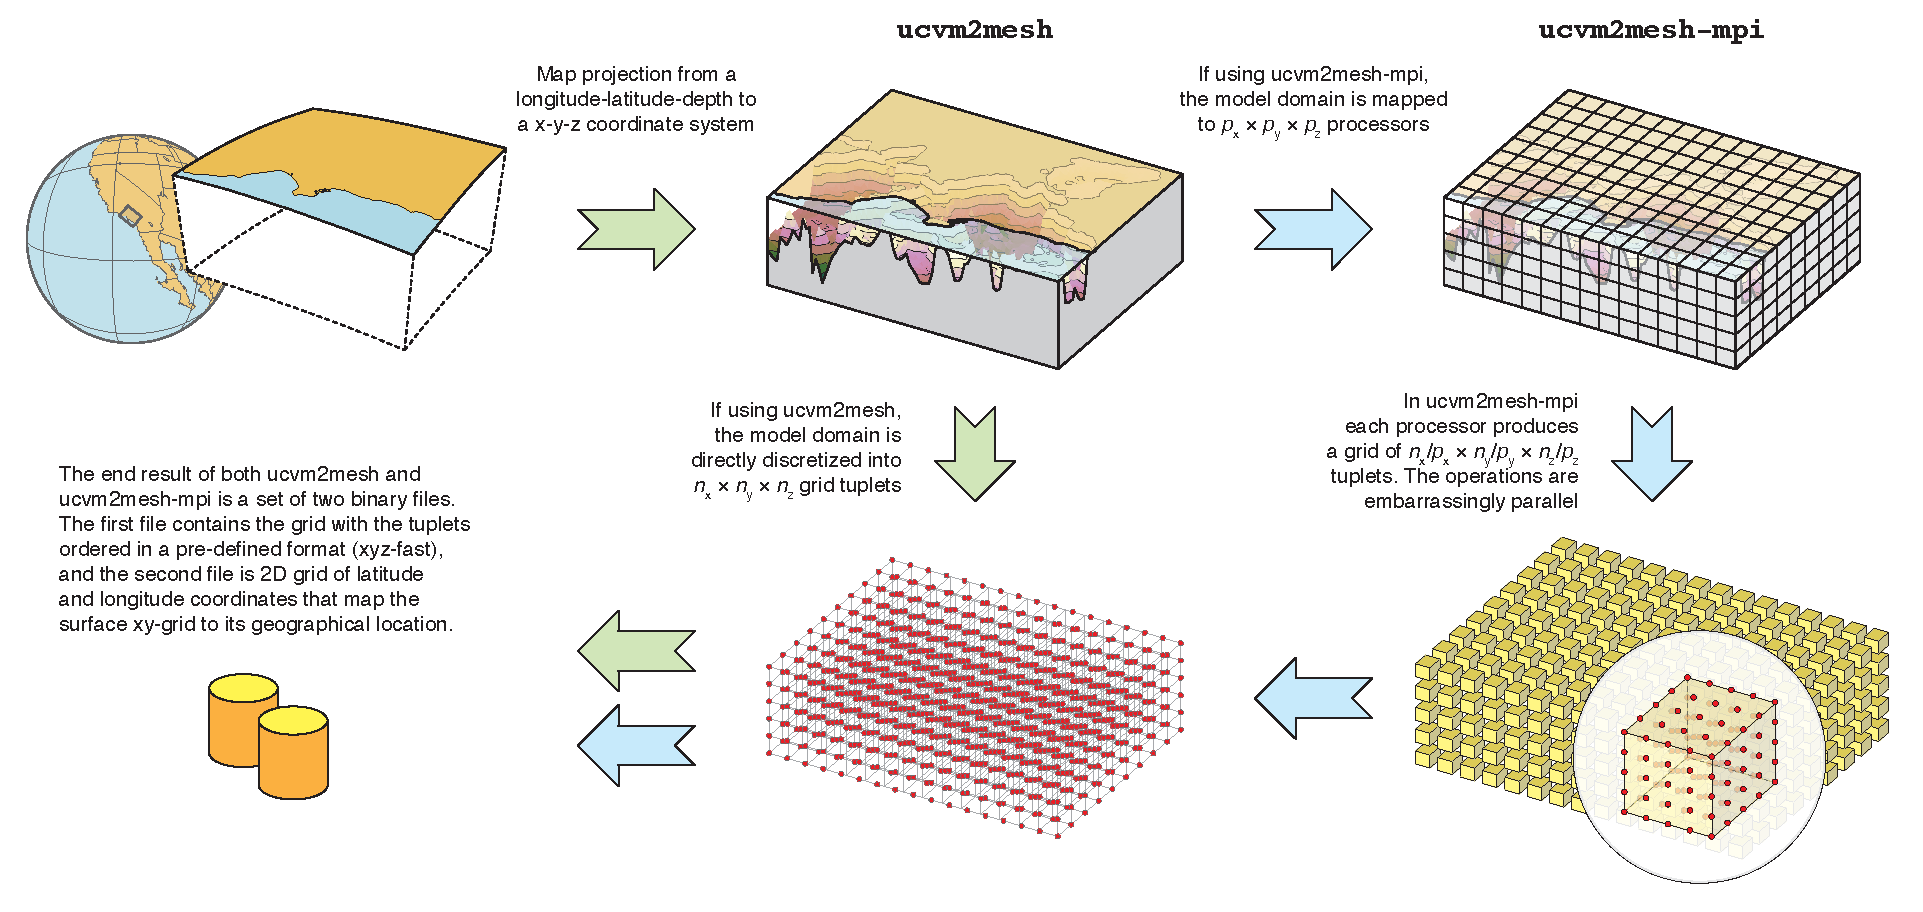
\includegraphics
		[width=\textwidth]
		{figures/pdf/ucvm-to-mesh}
	\caption{Construction of a structured grid with the programs \texttt{ucvm2mesh} (green arrows) and \texttt{ucvm2mesh-mpi} (blue arrows). An important aspect of the gridding process is that the discretized information payload (\vs{}, \vp{}, and $\rho$) is stored at the grid points. That is, the querying and assignment process has a 1-to-1 mapping between the queried point and the grid node of the mesh.}
	\label{fig:meshing}
\end{figure*}


\subsection{Creating Structured 3D Meshes}

The framework may be utilized to generate a structured uniform mesh in a format consistent with that used by the AWP-ODC simulation codes with the program \texttt{ucvm2mesh}.

Construction of a mesh proceeds as shown in Figure \ref{fig:meshing}. The user specifies a two-dimensional map projection (such as UTM-11), a latitude and longitude geographic anchor point, mesh cell dimensions ($n_x$, $n_y$, $n_z$) along the x,y and z axis (where x-y is in the plane of the projection and z is vertical), step size $d_x$ in meters within the projected space, and rotation angle within the map projection. Additionally, the user provides a list of CVMs to query, and these models are tiled in the same manner as was described in the previous section.

The program \texttt{ucvm2mesh} projects the geographic coordinates of the Earth's surface into the map projection, placing the origin of the mesh as the anchor point and discretizing the volume according to the provided dimensions and step size. For each point in the projected volume, \texttt{ucvm2mesh} determines the analous geographic point in terms of (latitude, longitude, depth) and queries the underlying CVMs for material properties. These material properties are then assigned to the mesh point. A minimum $V_s$ floor can be set to bound low velocities.

Four binary mesh formats are supported: IJK-12, IJK-20, IJK-32, and SORD. The first three formats are mesh variants used by AWP-ODC (NOTE: cite) and the last format is used by SORD (NOTE: cite and check if still true). For IJK-12 formatted meshes, the output is a binary file consisting of a list of $n_xn_yn_z$ tuples. Each tuple contains three single precision floating point values $(V_p. V_s, \rho)$, representing the material properties for a point in the mesh, with the mesh coordinates given implicitly by the position of the tuple in the list. The tuples are arranged in x-y-z order, with units of meters per second. 

Similarly, the IJK-20 format adds two quality factors, $Q_p$ and $Q_s$, so that each tuple contains $(V_p. V_s, \rho, Q_p, Q_s)$. The quality factors are derived from the $V_s$ by the following equations (NOTE: cite where these came from - AWP?):
\begin{equation}
Q_s = \frac{50 V_s}{1000}, \qquad \qquad Q_p = 2 Q_s
\end{equation}
The IJK-32 format extends IJK-20 further by adding the three four-byte integers $(i,j,k)$ to each tuple, explicitly representing the index coordinate of the grid cell within the mesh. In this latter case, each tuple contains $(i, j, k, V_p. V_s, \rho, Q_p, Q_s)$.

To facilitate the construction of very large meshes, the framework offers a parallel version of the mesher named \texttt{ucvm2mesh-mpi}. This MPI program operates analogously to that of the serial version. Spatial decomposition is performed by mapping subblocks of the meshing region to individual processors for extraction. The mapping is specified by providing a processor grid to the program at startup, which specifies the number of processors along each dimension. If the meshing region is sized $(n_x, n_y, n_z)$ grid points along each dimension, and the processor grid is specified as $(p_x, p_y, p_z)$, then each processor is assigned $(n_x/p_x, n_y/p_y, n_z/p_z)$ grid points. The only constraint in the mapping is that the processor count along a particular dimension must divide evenly into the number of grid points along that dimension. Once the region has been decomposed in this manner, extraction of material properties is an embarrassingly parallel operation.  


\begin{figure*}[ht!]
	\centering
	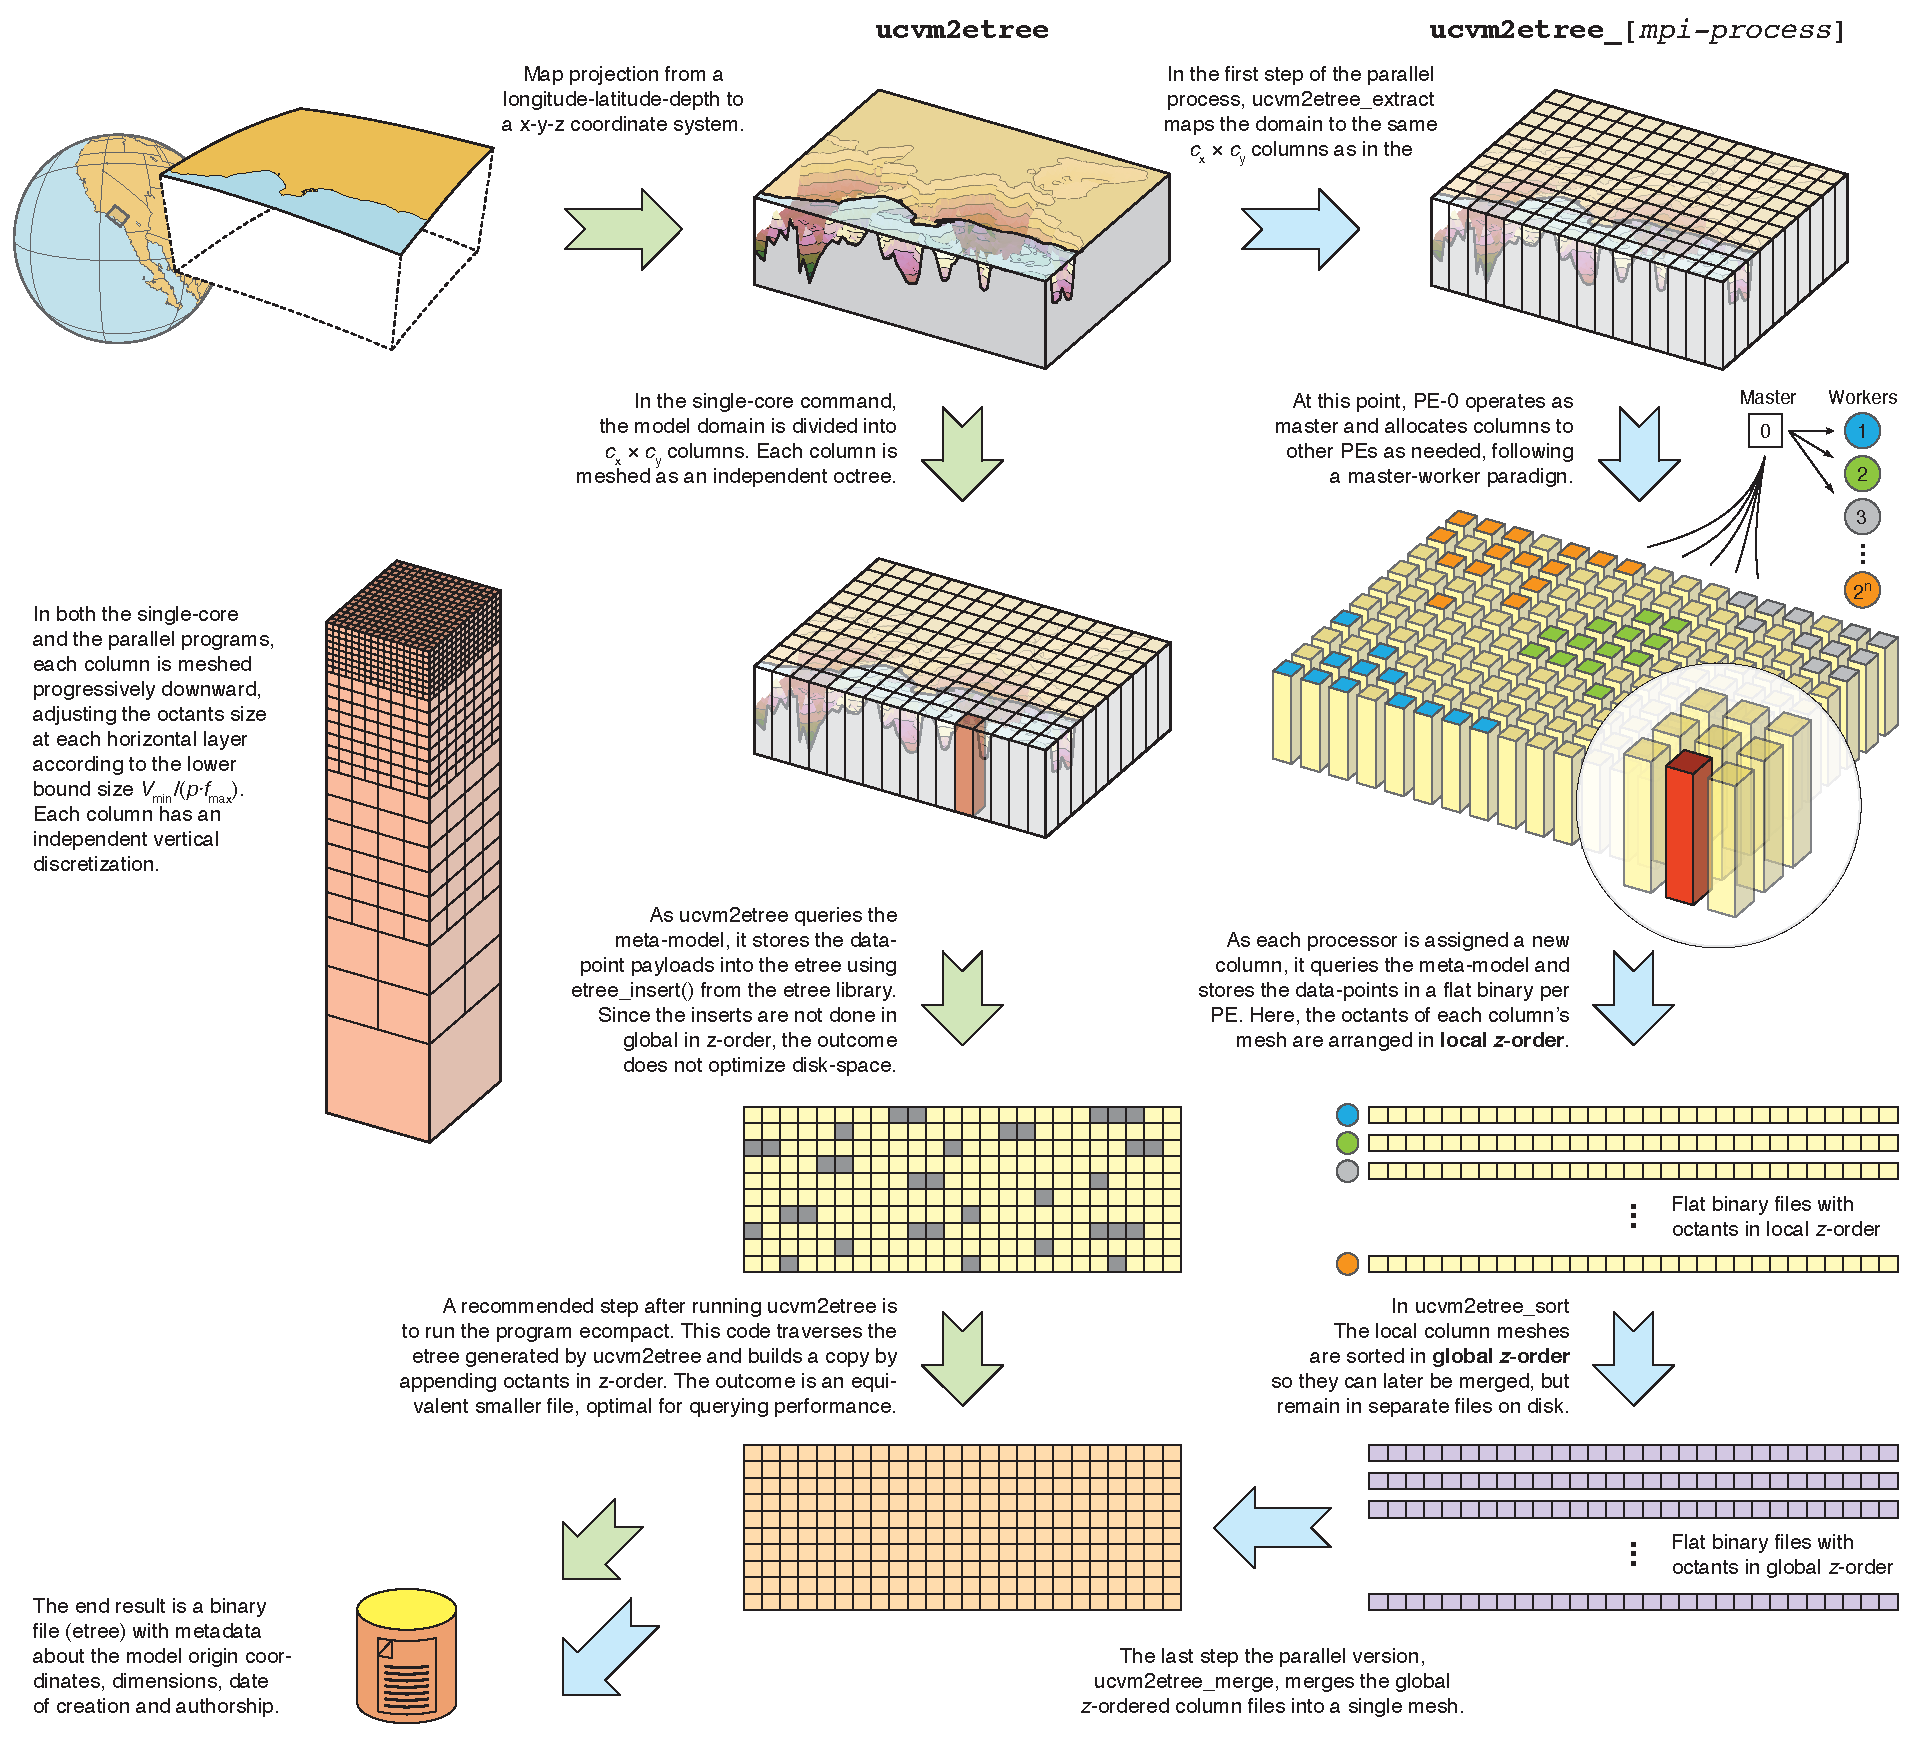
\includegraphics
		[width=\textwidth]
		{figures/pdf/ucvm-to-etree}
	\caption{Construction of an pseudo-unstructured mesh in the Etree database format using the program \texttt{ucvm2etree} and its MPI equivalent processes \texttt{ucvm2etree\_extract}, \texttt{ucvm2etree\_sort} and \texttt{ucvm2etree\_merge}. An important aspect of the meshing-to-etree process is that the discretized information payload (\vs{}, \vp{}, and $\rho$) is stored at the octants in the octree structure. The querying and assignment process mapps the information queried at the center of each octant to the whole volume enclosed by the octant.}
	\label{fig:etrees}
\end{figure*}
% ---------------------------------------------------------------------------------------------


\subsection{Creating Etree Databases}

The framework may also be utilized to generate a structured octree in the Etree database format (NOTE: cite Euclid Etree) using the command-line program \texttt{ucvm2etree}. Two Etree database formats are supported: the Hercules format, and the SCEC format. These two formats differ in the map projection used to discretize the domain. The Hercules format utilizes a projection that is a bilinear interpolation of a bounding box specified in geographical coordinates. The SCEC format supports any map projection available in the Proj.4 projection library.

For the purposes of this discussion, we shall describe the generation of a Hercules format Etree database. Construction of such an Etree proceeds as shown in Figure \ref{fig:etrees}. The user specifies the extents of the Etree by describing the x-y-z dimensions of the domain in meters, as well as providing the geographical coordinates of a bounding box on the Earth's surface. This surface bounding box is mapped to the x-y plane of the domain using bilinear interpolation. The z dimension of the domain is interpreted as depth from the free surface. In this way, any $(x,y,z)$ coordinate in the domain may be transformed to a $(latitude, longitude, depth)$ coordinate relative to the Earth's surface. It is assumed that the user has pre-computed the domain dimensions such that they reflect the actual distances in the geographic bounding box (using any projection or spheroid model of their choosing). Note, however, that the octree format places restrictions on the possible valid domain sizes (NOTE: cite Euclid etree or other paper that describes this format in greater detail).

This domain is then spatially decomposed at a coarse-grained level, dividing the volume into a two-dimensional logical grid of rectangular cuboids (columns) aligned with the x-y plane of the original domain, with each column having fixed size. This decomposition assists in parallelization since the material properties for a particular column can be extracted independently from the others. The number of columns in this logical grid is selectable by the user, subject to two constraints to preserve the octree format. First, the length and width of the columns must be equal. Second, the number of columns along the x and y axis must be a power of two.

With this coarse decomposition complete, each column of the original domain may then be processed in sequence by \texttt{ucvm2etree}, or in parallel, as is the case with the MPI version of this utility. To extract the material properties for a column, the program further decomposes the column into a collection of octants, bilinearly interpolates the $(x,y,z)$ coordinate of each octant to geographic coordinates, and then queries the user-provided list of velocity models to determine the $(V_p, V_s, \rho)$ payload for each. The octants are processed in a top-down fashion, starting at the surface and ending at the maximum depth of the domain. Filled octants are inserted into the Etree database via the Etree API.

This fine-grain decomposition into octants is an adaptive process that depends on the shear-wave velocities, $V_s$, encountered within that column as well as four parameters provided by the user: $V_{min}$, a floor $V_s$ for purposes of bounding octant sizes to a minimum size, $f_{max}$, the maximum simulation frequency to support, $p$, the desired points per wavelength, and $s_{max}$, the maximum octant size to allow. From these parameters, the program first determines the range of octant sizes to allow within the column. The upper bound is determined by the following relation:
\begin{equation}\label{eq:octant_upper}
s_{upper} = min(l_c, s_{max})
\end{equation}
Where $l_c$ is the column length. The lower bound is given by (NOTE: where did this come from?):
\begin{equation}\label{eq:octant_lower}
s_{lower} = \frac{V_{min}}{p f_{max}}
\end{equation}
As the octree format places constraints on valid octant sizes, these two bounds are then normalized with the relation:
\begin{equation}\label{eq:octant_size}
s_{octant} = \frac{l_{d}}{ 2^{\left( \left\lceil \log_{2}(\frac{l_{d}}{s}) \right\rceil \right)} }
\end{equation}
The variable $l_{d}$ is the domain length (longest side). The variable $s$ is the size to normalize, either $s_{upper}$ or $s_{lower}$, corresponding to the upper and lower bounds, respectively.

With these bounds established, the program successively queries two-dimensional slices of octants, starting at the column surface and stepping downward to greater depths. Inititially, the octants are of size $s_{lower}$ (maximum resolution), however, the octants may be resized based on the actual $V_s$ values encountered within a slice. After each slice is queried, the minimum $V_s$ found within is inserted into equation (\ref{eq:octant_lower}) and then normalized with (\ref{eq:octant_size}) to yield an updated octant size. If this new size differs from the current size, yet falls within the $s_{lower}$ and $s_{upper}$ bounds, and this size fits in the remaining vacant space of the octree, the slice is re-queried at the new size. Otherwise, the slice of octants is inserted into the Etree database.

This adaptive refinement continues as the program steps down through the column. As $V_s$ velocities typically increase with depth, the program will tend to select larger octant sizes as it proceeds deeper into the column. This refinement algorithm ensures that each column is extracted at a resolution which supports the maximum simulation frequency, while at the same time allowing for considerable space savings at depth.

The MPI implementation of \texttt{ucvm2etree} consists of a workflow with three programs: \texttt{ucvm2etree\_extract}, \texttt{ucvm2etree\_sort}, and \texttt{ucvm2etree\_merge}. The program \texttt{ucvm2etree\_extract} performs the same spatial decomposition and velocity model querying as described above, with the change that each column is extracted independently by each processor and the octants are temporarily saved to disk in flat binary files. The program \texttt{ucvm2etree\_sort} locally sorts the octants of each column by their location code, which is a function defined as a space-filling curve. The last program in the workflow, \texttt{ucvm2etree\_merge}, performs a merge sort of the locally sorted columns, such that rank 0 inserts the ordered octants one at a time into the Etree database. Since the octants are globally sorted at this point, the insertion is simply an append operation. This scheme, while more complicated than the sequential program, allows extraction to occur in parallel while utilizing the most efficent insertion method currently provided by the Etree library.

\subsection{Miscellaneous Features}

The UCVM framework encompasses a set of minor features intended to support typical use cases, as well as to enhance ease-of-use. These minor features are described in greater detail in the following sections.

\subsubsection{Querying $V_s$ Iso-surfaces}

The basin structure of a velocity model may be extracted using the \texttt{basin\_query} command. This program accepts a shear wave velocity threshold $V_{thresh}$, a step interval $d_z$ along the vertical axis, one or more velocity models, and a list of (latitude, longitude) geographic coordinates. The program begins by tiling the velocity models to form the meta-model. Then, for each input coordinate, the meta-model is queried at a sequence of depths, starting at the surface and proceeding downward with step size $d_z$ meters until either the configured $V_{thresh}$ is exceeded or a maximum search depth is reached. The shallowest depth at which this transition occurs, or the maximum depth if no transition was found, is reported to the user. An MPI version of this command, \texttt{basin\_query\_mpi}, is provided to quickly generate maps for large sets of coordinates.

\subsubsection{Visualization}

The framework provdes a simple mechanism for visualizing slices and iso-surfaces from any configured velocity model, based on the scripting language Python and the Python modules \texttt{matplotlib} (with the basemap toolkit) (NOTE: cite url), \texttt{numpy} (NOTE: cite url), and \texttt{pyproj} (NOTE: cite url). These Python scripts function as wrappers to the basic single-core commands explained previously.

Plots of horizontal and vertical slices may be generated with the \texttt{horizontal\_slice.py} and \texttt{cross\_section.py} scripts, respectively. Horizontal slices are oriented by a simple bounding box specified in geographic coordinates at a specified depth. Cross sections are oriented by two geographic endpoints and a depth range. In both cases, the slice region is discretized into a grid and each grid point is queried from the velocity model(s). The value plotted may be any one of the three material properties $V_p$, $V_s$, and $\rho$, or the Poisson ratio, $\nu$, of the velocities, given by:
\begin{equation}
\nu = \frac{V_p}{V_S}
\end{equation}
In addition, basin maps for $V_s = 1000$ m/s and $V_s = 2500$ m/s may be plotted using the \texttt{z10.py} and \texttt{z25.py} scripts, respectively. These operate analogously to the \texttt{basin\_query} command described previously. Lastly, generation of $V_{s30}$ maps is supported with the \texttt{vs30.py} script. In all cases, the output images are saved to disk in Portable Network Graphics (PNG) format.

\subsubsection{Small-scale Heterogeneities}

The last decade has seem a tremendous growth on high performance computing and applications dedicated to earthquake ground motion simulations which is leading the charge toward performing deterministic simulations at high frequencies of engineering interest (\fmax{} 0--10 Hz). With increasing simulation frequencies, seismic velocity models must not only be accurate representations of a region's crustal structure at the geologic scale and represent the geotechnical characteristics of basins and deposits, but should also provide for the adequate representation of the scattering characteristics of the typical heterogeneities observed in geomaterials. To this end, UCVM provides a mechanism for incorporating small-scale heterogeneities into any underlying velocity model. This mechanism is implemented as a post-processing step to meshing, such that a structured mesh of material properties is first produced using \texttt{ucvm2mesh} and this mesh is subsequently modified to incorporate the small-scale heterogeneities.

Introduction of small-scale heterogeneities begins by constructing an identically sized mesh using the command \texttt{ssh\_generate} (NOTE: cite Olsen). However, the payload of the grid points in this mesh are the perturbations (with a normalized amplitude) to apply to each of the three material properties $V_p$, $V_s$, and $\rho$ of the original mesh. Then, the command \texttt{ssh\_merge} is used to iterate through the cells of the two meshes and add the heterogeneities multiplied by a user-defined scaling factor to the model according to the following relation:
\begin{equation}
Perturbation \qquad calculation \qquad TBD
\end{equation}
(NOTE: Explain the terms here). Note that introduction of the heterogeneities is accomplished by applying the scaled perturbation to the slowness of the underlying mesh velocities, and then converted back to the seismic velocity. 

\subsubsection{Easy Install Utility}
\label{sec:easy.install}

TBD
